\chapter{Evaluación}
\label{cap:evaluacion}
Una vez terminado el desarrollo de AdaptaMaterialEscolar 2.0, llevamos a cabo una evaluación para cumplir con nuestro objetivo principal: confirmar si nuestro proyecto resultaba útil para los docentes que necesitaban realizar adaptaciones curriculares para sus estudiantes en cualquier etapa académica. Con el propósito de realizar una valoración detallada, nos enfocamos en evaluar varios aspectos de nuestro proyecto. Estos incluían el diseño de la interfaz, la usabilidad del sistema en su totalidad, cada funcionalidad de manera independiente y las posibles mejoras que podrían implementarse en el futuro.

A continuación se explica el diseño de la evaluación (Sección \ref{sec:disenyoEvaluacion}), los resultados obtenidos tras la evaluación (Sección \ref{sec:resultadosEvaluacion}) y las conclusiones obtenidas (Sección \ref{sec:conclusionesEvaluacion}).

\section{Diseño}\label{sec:disenyoEvaluacion}
Con el fin de permitir a los usuarios finales evaluar nuestra aplicación, creamos un examen de prueba y una hoja de apuntes sobre las asignaturas de conocimiento del medio y matemáticas.
Para facilitar la evaluación y el análisis de los resultados de nuestra aplicación web, creamos una encuesta\footnote{\url{https://docs.google.com/forms/d/e/1FAIpQLSdg7mGUfGBW5LoGIWulEUq-vhloL5rlkU_aIZCUzpqiJp164A/viewform?usp=sf_link}} en Google Forms dirigida a los usuarios finales. Durante la evaluación, los usuarios experimentaban directamente con las diversas funcionalidades, tratando de replicar el examen y la hoja de apuntes proporcionados.

La evaluación ha constado de 3 partes y ha sido diseñada para que se realice en aproximadamente 45 minutos. Las partes de la evaluación han sido las siguientes: la creación de un modelo de examen, la elaboración de unos apuntes adaptados y una evaluación general de la aplicación. En las dos primeras partes, los usuarios han debido realizar distintas tareas. Para cada tarea, se ha proporcionado una explicación detallada de cómo realizarla, junto con una imagen que muestra cómo quedaría el documento una vez completada. Al finalizar cada tarea, se han planteado 3 preguntas para evaluarla. Una vez completadas las dos primeras partes de la evaluación, se ha presentado un cuestionario compuesto por 10 preguntas, con el objetivo de evaluar la facilidad de uso de la aplicación. Para finalizar, se han planteado una serie de preguntas de respuesta abierta para conocer la opinión de los usuarios sobre la herramienta. Después de crear cada parte de la evaluación (examen y apuntes), los usuarios han debido exportar el documento a PDF y subirlo a una carpeta de Google Drive.

En cuanto a las preguntas del cuestionario, se han estructurado de acuerdo con diferentes aspectos y han sido las siguientes:

\begin{itemize}
    \item \textbf{Preguntas generales}. Datos demográficos del usuario.
          \begin{itemize}
              \item ¿Cuántos años tienes?
              \item ¿Eres docente?
          \end{itemize}
    \item \textbf{Preguntas para no docentes}.
          \begin{itemize}
              \item ¿Eres estudiante de magisterio?
          \end{itemize}
    \item \textbf{Preguntas para docentes}. Recogen el nivel académico en el que imparten clase, si han realizado alguna adaptación curricular y, en caso afirmativo, cuantas veces.
          \begin{itemize}
              \item ¿Podrías decirnos en qué nivel del sistema educativo eres docente?
              \item ¿Has tenido que hacer alguna adaptación curricular no significativa?
              \item ¿Cuántas veces?
          \end{itemize}
    \item \textbf{Preguntas sobre funcionalidades}. Obtienen información sobre la
          dificultad de uso de cada funcionalidad y recopilar nuevas adaptaciones
          o mejoras que se desean para la aplicación.
          \begin{itemize}
              \item En general, estoy  satisfecho o satisfecha con la facilidad de completar esta tarea.
              \item En general estoy  satisfecho o satisfecha con la cantidad de tiempo que me ha llevado completar esta tarea.
              \item Estoy  satisfecho o satisfecha con la respuesta de la aplicación al realizar las acciones, sé lo que pasa en todo momento.
              \item En caso de la funcionalidad de pictotraductor también se han realizado las siguientes preguntas: ¿La traducción resultante te parece correcta? y ¿Qué cuestiones crees que son mejorables en la traducción o que no son correctas?
              \item En caso de la funcionalidad de generar resumen también se han realizado las siguientes preguntas: ¿El resumen resultante te parece correcto? y ¿Qué cuestiones crees que son mejorables en el resumen o que no son correctas?
          \end{itemize}
    \item \textbf{Preguntas sobre usabilidad}. El cuestionario utilizado para evaluar la usabilidad de un sistema es conocido como Escala de Usabilidad de un Sistema\footnote{\url{https://uxpanol.com/teoria/sistema-de-escalas-de-usabilidad-que-es-y-para-que-sirve/}}, (SUS, por sus siglas en inglés) y es ampliamente utilizado en este campo. El cuestionario consta de las siguientes preguntas:
          \begin{itemize}
              \item Creo que usaría esta aplicación frecuentemente.
              \item Encontré la aplicación innecesariamente compleja.
              \item Creo que la aplicación es fácil de usar.
              \item Creo que necesitaría la ayuda de una persona con conocimientos técnicos para usar la aplicación.
              \item Las funciones de la aplicación están bien integradas.
              \item Creo que la aplicación es muy confusa.
              \item Creo que la mayoría de la gente aprendería a usar la aplicación muy rápidamente.
              \item Encuentro la aplicación muy complicada de utilizar.
              \item Me siento confiado o confiada al utilizar la aplicación.
              \item Necesito aprender muchas cosas antes de poder utilizar la aplicación.
          \end{itemize}
    \item \textbf{Preguntas generales sobre la aplicación}. Recopilan la opinión de los usuarios sobre la aplicación:
          \begin{itemize}
              \item ¿Qué te ha parecido la aplicación?
              \item ¿Qué es lo que más te ha gustado?
              \item ¿Qué es lo que menos te ha gustado?
              \item ¿Echas de menos alguna funcionalidad?
              \item ¿Te sobra alguna funcionalidad?
              \item ¿Algo más que quieras añadir?
          \end{itemize}
\end{itemize}

En las preguntas en las que se requería asignar una puntuación como respuesta, utilizamos una escala Likert de 5 puntos. Esta escala iba del 1 al 5, donde el valor más bajo, 1, indicaba que el usuario estaba ``Muy en desacuerdo'' con la afirmación de la pregunta, y el valor más alto, 5, indicaba que el usuario estaba ``Muy de acuerdo''. Todos los aspectos de la encuesta, excepto la sección de usabilidad, fueron diseñados específicamente por nosotros para obtener información que consideramos relevante para el proyecto.

\section{Resultados}\label{sec:resultadosEvaluacion}
Finalmente, un total de 5 usuarios finales, todos ellos docentes de Educación Infantil, Primaria, Secundaria o Bachillerato, participaron en la evaluación de la aplicación web y respondieron a la encuesta. La puntuación final obtenida en las preguntas de usabilidad del Sistema de Usabilidad del Usuario (SUS) fue de 78.5, en una escala de 0 a 100. Esta puntuación indica que el sistema todavía requiere mejoras. Los detalles del cálculo se encuentran en la tabla \ref{tab:puntuacionSUS}.

\begin{table}[H]
    \resizebox{\textwidth}{!}{
        \begin{tabular}{cccc|c|c|}
            \cline{2-6}
            \multicolumn{1}{l|}{}                      & \multicolumn{1}{c|}{\textbf{Usuario 1}} & \multicolumn{1}{c|}{\textbf{Usuario 2}} & \textbf{Usuario 3}        & \textbf{Usuario 4}      & \textbf{Usuario 5}      \\ \hline
            \multicolumn{1}{|c|}{\textbf{Pregunta 1}}  & \multicolumn{1}{c|}{5}                  & \multicolumn{1}{c|}{4}                  & 4                         & 5                       & 2                       \\ \hline
            \multicolumn{1}{|c|}{\textbf{Pregunta 2}}  & \multicolumn{1}{c|}{1}                  & \multicolumn{1}{c|}{2}                  & 2                         & 1                       & 3                       \\ \hline
            \multicolumn{1}{|c|}{\textbf{Pregunta 3}}  & \multicolumn{1}{c|}{4}                  & \multicolumn{1}{c|}{4}                  & 4                         & 5                       & 3                       \\ \hline
            \multicolumn{1}{|c|}{\textbf{Pregunta 4}}  & \multicolumn{1}{c|}{5}                  & \multicolumn{1}{c|}{1}                  & 1                         & 1                       & 2                       \\ \hline
            \multicolumn{1}{|c|}{\textbf{Pregunta 5}}  & \multicolumn{1}{c|}{5}                  & \multicolumn{1}{c|}{4}                  & 4                         & 5                       & 2                       \\ \hline
            \multicolumn{1}{|c|}{\textbf{Pregunta 6}}  & \multicolumn{1}{c|}{2}                  & \multicolumn{1}{c|}{2}                  & 2                         & 1                       & 3                       \\ \hline
            \multicolumn{1}{|c|}{\textbf{Pregunta 7}}  & \multicolumn{1}{c|}{5}                  & \multicolumn{1}{c|}{4}                  & 5                         & 4                       & 4                       \\ \hline
            \multicolumn{1}{|c|}{\textbf{Pregunta 8}}  & \multicolumn{1}{c|}{1}                  & \multicolumn{1}{c|}{5}                  & 1                         & 1                       & 2                       \\ \hline
            \multicolumn{1}{|c|}{\textbf{Pregunta 9}}  & \multicolumn{1}{c|}{5}                  & \multicolumn{1}{c|}{5}                  & 5                         & 5                       & 3                       \\ \hline
            \multicolumn{1}{|c|}{\textbf{Pregunta 10}} & \multicolumn{1}{c|}{1}                  & \multicolumn{1}{c|}{1}                  & 1                         & 4                       & 2                       \\ \hline
            \multicolumn{1}{|c|}{\textbf{Resultado}}   & \multicolumn{1}{c|}{85}                 & \multicolumn{1}{c|}{75}                 & \multicolumn{1}{c|}{87,5} & \multicolumn{1}{c|}{90} & \multicolumn{1}{c|}{55} \\ \hline
            \multicolumn{1}{l}{}                       & \multicolumn{1}{l}{}                    & \multicolumn{1}{l}{}                    & \multicolumn{1}{l|}{}     & \textbf{Media:}         & \textbf{78,5}           \\ \cline{5-6}
        \end{tabular}
    }
    \caption{Resultado del cuestionario SUS}
    \label{tab:puntuacionSUS}
\end{table}

En relación a las preguntas sobre las funcionalidades individuales, los resultados revelan que, en términos generales, los usuarios se encuentran satisfechos con la aplicación, tal como se ilustra en la Figura \ref{fig:graficaPreguntasFuncionalidades}. Al profundizar en el análisis, se observa que los usuarios consideran que las funcionalidades relacionadas con la creación de ejercicios son más fáciles e intuitivas, como se muestra en la Figura \ref{fig:graficaComparativaEjerciciosApuntes}. En resumen, todas las respuestas indicaron que el proyecto resultó muy útil para los profesores y manifestaron su interés en que se continuara desarrollando en el futuro.

\begin{figure}[H]
    \centering
    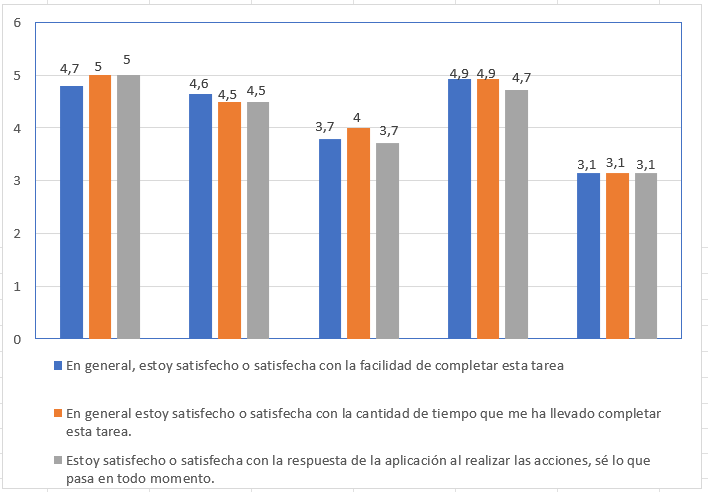
\includegraphics[width=0.75\textwidth]{Evaluacion/GraficaPreguntasFuncionalidades.png}
    \caption{Gráfica de resultados de Funcionalidades.}
    \label{fig:graficaPreguntasFuncionalidades}
\end{figure}

\begin{figure}[H]
    \centering
    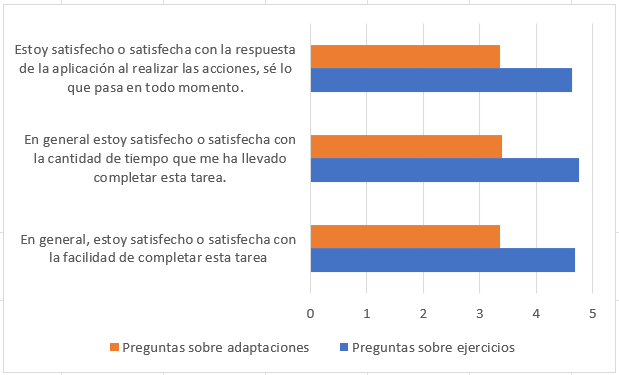
\includegraphics[width=0.75\textwidth]{Evaluacion/GraficaComparativaEjerciciosApuntes.png}
    \caption{Gráfica comparativa entre ejercicios y apuntes.}
    \label{fig:graficaComparativaEjerciciosApuntes}
\end{figure}

\section{Conclusiones}\label{sec:conclusionesEvaluacion}
Tras evaluar la aplicación web AdaptaMaterialEscolar 2.0, podemos determinar que su recepción por parte de los usuarios finales ha superado nuestras expectativas. Hemos logrado desarrollar una herramienta para docentes que cumple con éxito sus necesidades al facilitar la adaptación de material escolar. La usabilidad del sistema, con una puntuación de 78.5 sobre 100, indica que existe margen de mejora si continuamos colaborando con nuevos usuarios. No obstante, en su estado actual, la aplicación ofrece una experiencia de usuario más que satisfactoria.

En conclusión, el proyecto ha sido un acierto y existe una necesidad real de seguir desarrollándolo y mejorándolo para abarcar las diversas solicitudes de los docentes y las asignaturas de los centros académicos que podrían beneficiarse de su uso.

Aunque el proyecto despertó más interés del esperado entre el profesorado, el número de evaluaciones obtenidas fue limitado. Para obtener conclusiones más significativas, se debería contactar con más docentes para recabar sus evaluaciones y propuestas de mejora futura para la aplicación.